
\section{Study of Parallel Workload~\Rmnum{1}}
%\section{Identify the ``Bully"}
\label{sec:workload-1}

The study of parallel workload~\Rmnum{1} consists of two parts. Firstly, we analyze the over-all network performance when Workload~\Rmnum{1} is running under different placement and routing configurations. Secondly, we isolate each application from the workload, analyze its performance by scrutinizing the traffic going through the routers that serve each job. The analysis allows us to identify the ``bully" in the workload. 



\subsection{Network Performance Analysis}
\label{sec: workload-1 network analysis}

We study the network performance under different placement and routing configurations by analyzing the traffic going through the routers and their saturated time. 
The distribution of traffic over the network can reveal the loading situation, 
indicating whether the network is load-balanced or not. 
The saturated time can indicate the congestion situation on certain part of the network. 


\begin{figure*}[t!]
    \centering
    \begin{subfigure}[t]{0.32\textwidth}
        \centering
        \includegraphics[height=1.8 in]{wkld/gc-traffic}
        \caption{Global Channel Traffic}
        \label{fig:global-channel-traffic}
    \end{subfigure}\hfill
    \hspace{1em}%
    \begin{subfigure}[t]{0.32\textwidth}
        \centering
        \includegraphics[height=1.8 in]{wkld/lc-traffic}
        \caption{Local Channel Traffic}
        \label{fig:local-channel-traffic}
    \end{subfigure}\hfill
    \hspace{1em}%
    \begin{subfigure}[t]{0.32\textwidth}
        \centering
        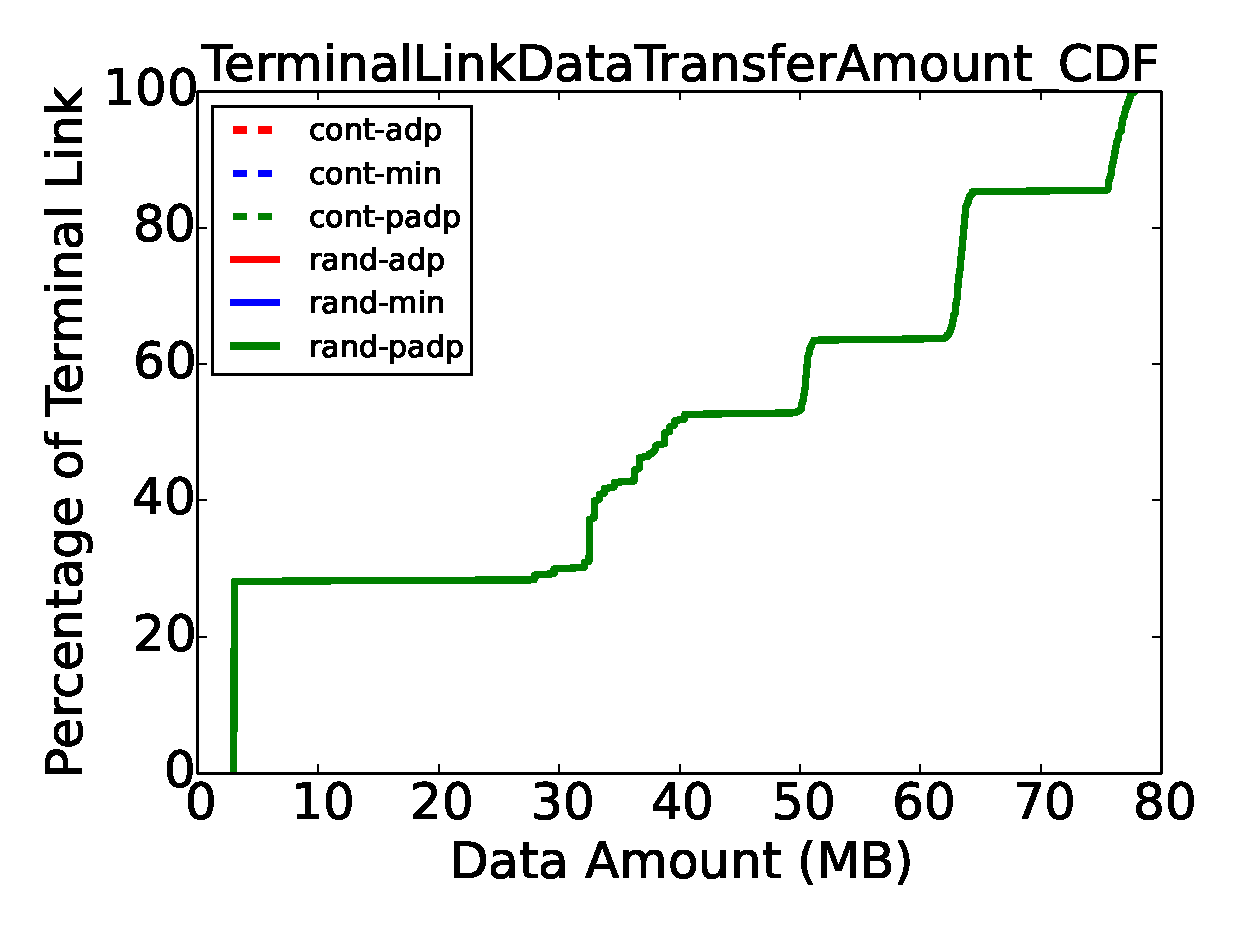
\includegraphics[height=1.8 in]{wkld/tl-traffic}
        \caption{Terminal Link Traffic}
        \label{fig:terminal-link-traffic}
    \end{subfigure}\\

    \centering   
    \begin{subfigure}[t]{0.32\textwidth}
        \centering
        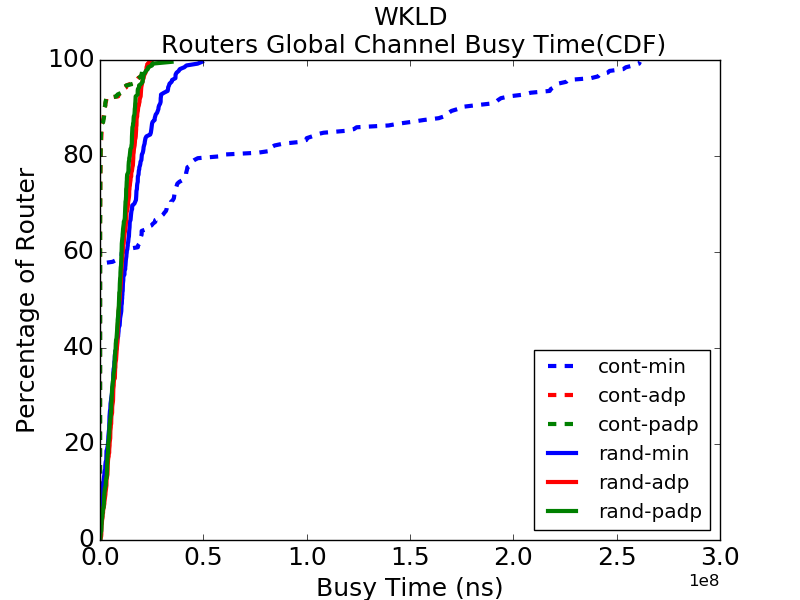
\includegraphics[height=1.8 in]{wkld/gc-stime}
        \caption{Global Channel Saturated Time}
        \label{fig:global-channel-stime}
    \end{subfigure}\hfill
     \hspace{1em}%
    \begin{subfigure}[t]{0.32\textwidth}
        \centering
        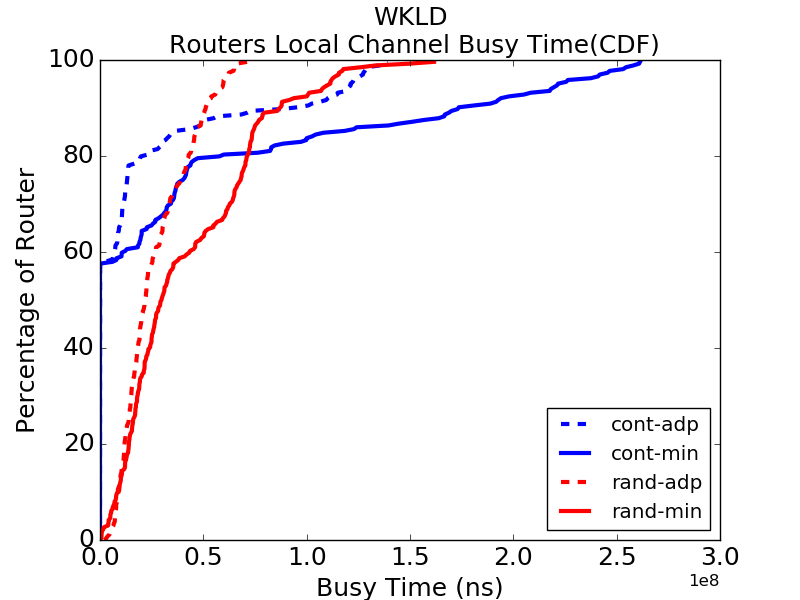
\includegraphics[height=1.8 in]{wkld/lc-stime}
        \caption{Local Channel Saturated Time}
        \label{fig:local-channel-stime}
    \end{subfigure}\hfill
    \hspace{1em}%
    \begin{subfigure}[t]{0.32\textwidth}
        \centering
        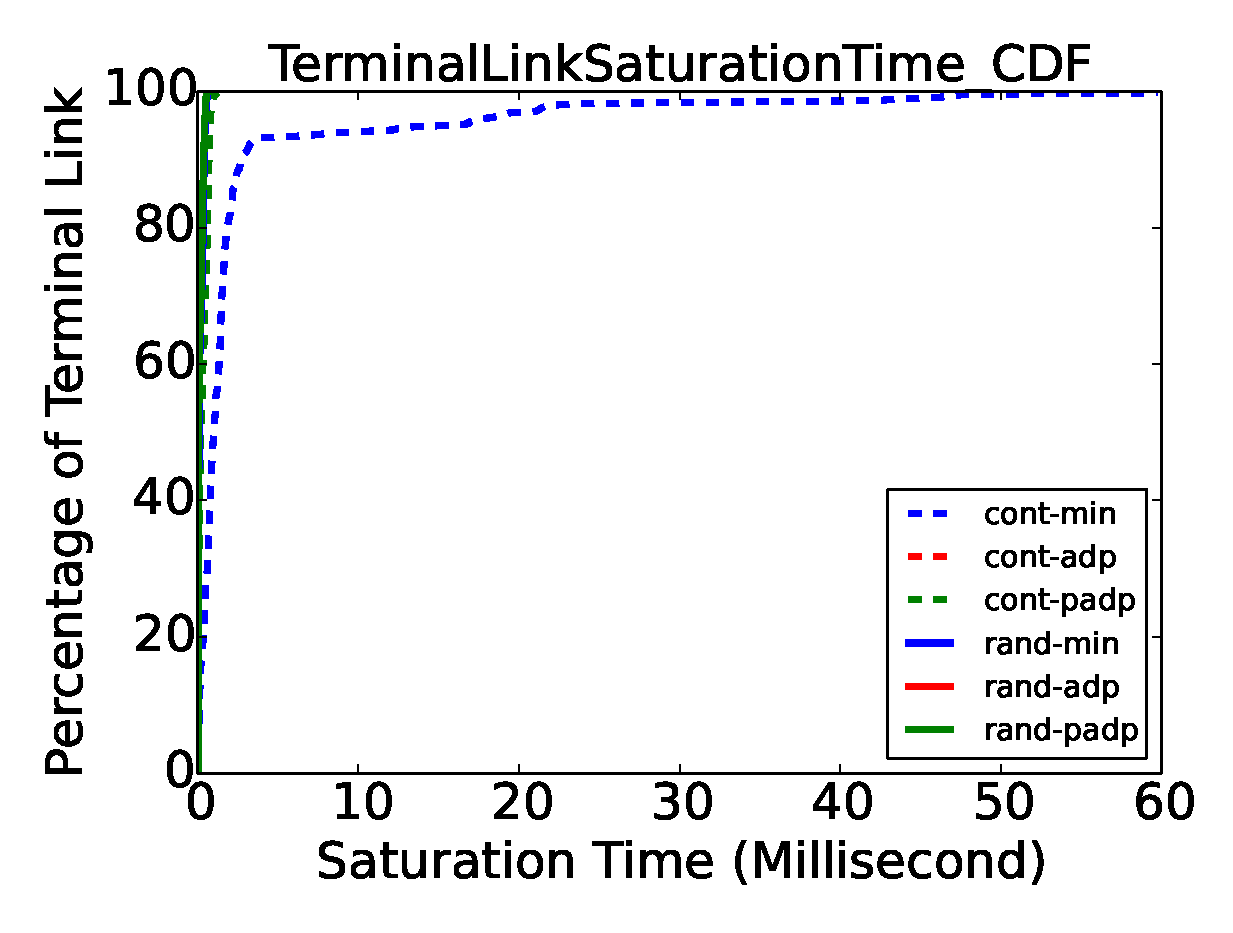
\includegraphics[height=1.8 in]{wkld/tl-stime}
        \caption{Terminal Link Saturated Time}
        \label{fig:terminal-link-stime}
    \end{subfigure}%
   \caption{The aggregate traffic and saturated time of the dragonfly network when Workload~\Rmnum{1} running under six different placement and routing configurations. ``CA" and ``CPA" performs comparably, the corresponding lines are overlapped. }
   \label{fig:wkld-network-traffic-stime}
\end{figure*}


Figure~\ref{fig:wkld-network-traffic-stime} shows the aggregate traffic for terminal links, local and global channels 
as well as the corresponding saturated time when 
Workload~\Rmnum{1} is running on the dragonfly network with six different placement and routing configurations. 
When contiguous placement coupled with minimal routing(CM) is in use, 
all the traffic are confined within the contiguously allocated groups, 
causing congestion on some routers along certain shortest paths from the source to the destination. 
The congested routers are over-loaded with high volume of traffic going through their local and global channels, 
shown as the blue dashed line in Figure~\ref{fig:global-channel-traffic} and~\ref{fig:local-channel-traffic}. 
In the meanwhile, the corresponding saturated time of their local and global channels are also the highest compared with other configurations, 
shown as the blue dashed line in Figure~\ref{fig:global-channel-stime} and Figure~\ref{fig:local-channel-stime} .



When contiguous placement coupled with progressive adaptive routing (CPA) is in use, 
the traffic would take non-shortest paths via intermediate routers to void congestion. 
The congested routers along the shortest paths will not suffer the high volume of traffic as they used to. 
The traffic through local and global channels are greatly reduced, 
shown as the green dashed line in Figure~\ref{fig:global-channel-traffic} and~\ref{fig:local-channel-traffic}. 
The corresponding saturated time on local and global channels also drop a lot, 
indicating the congestion are alleviated by using progressive adaptive routing. 
The adaptive routing performs comparably compared with progressive adaptive routing, 
thus CA is overlapped with CPA in the all the figures above.



Random placement policy performs comparably with three different routing policies.
Random placement can uniformly distribute MPI ranks over the network, 
balance the traffic load over the network. 
Shown as the solid lines in Figure~\ref{fig:global-channel-traffic} and~\ref{fig:local-channel-traffic}, 
no router suffers exceptional high volume of traffic on its local and global channels. 
When the random placements coupled with minimal routing (RM), 
the packets can avoid unnecessary intermediate forwarding as introduced by (progressive) adaptive routing, thus generating less traffic. 
The blue solid line(RM) is lower than the red and green solid line (RA, RPA) in Figure~\ref{fig:global-channel-traffic} and~\ref{fig:local-channel-traffic}. 



Due to the same reason, 
no router suffers exceptionally long saturated time on their global channels when random placement coupled (progressive) adaptive are in use, 
shown as red and green solid lines in Figure~\ref{fig:global-channel-stime} and~\ref{fig:local-channel-stime}. 
However, when random placement is couple with minimal routing, 
the saturated time on certain routers along the shortest paths would increase, 
shown as the prolonged blue solid line in Figure~\ref{fig:global-channel-stime} and~\ref{fig:local-channel-stime}. 
Since the minimal routing always chooses the shortest paths, 
increasing the possibility of congestion along those paths. 


%terminal link traffic and busy time explanation
Figure~\ref{fig:terminal-link-traffic} is for the purpose of symmetry, 
it shows the traffic per rank (aka traffic through terminal links), 
which stay the same when different placement and routing configurations are in use. 
All six lines are overlapped in Figure~\ref{fig:terminal-link-traffic}. 
However, due to the traffic changes on local and channels, 
the saturated time of terminal links will experience variability when different routing policies are in use, as shown in Figure~\ref{fig:terminal-link-stime}. 
When contiguous placement coupled with minimal routing(CM), 
the accumulated congestion on local and global channels cause extremely long saturated time on the terminal links, 
shown as the blue dashed line in Figure~\ref{fig:terminal-link-stime}. 
This again manifests the severe congestion caused by using contiguous placement and minimal routing. 


%===========================================================
%from the workload perspective to study the network performance. 
The efficiency of the workload communication is another perspective to evaluate the network performance. 
The average communication time spent by all MPI ranks when Workload~\Rmnum{1} is running under different placement and routing configurations shown in Table~\ref{tab:wkld-commtime}. 
The random placement policy performs comparably with all routing policies (RM, RA and RPA). They outperform all contiguous placement configurations (CM, CA and CPA). The contiguous placement coupled with minimal routing (CM) results in highest communication time. When coupled with (progressive) adaptive routing (CA, CPA), the average communication time can be greatly reduced. When random placement is in use, the workload communication efficiency can be further improved. 


\begin{table}[ht]
\begin{center}
\caption{Average communication time by all MPI ranks when Workload I is running on the dragonfly network under six different placement and routing configurations.} 
\label{tab:wkld-commtime}
\begin{tabular}{l c c c c c c }
\toprule % Top horizontal line
\toprule
&\multicolumn{6}{c}{Placement and Routing Configurations} \\ 
\cmidrule(l){2-7}
          & CM & CA & CPA & RM & RA & RPA \\ % Column names row
\midrule % In-table horizontal line
Time(ms)  & 476  & 300  & 301  & 255  & 265  & 264  \\ % Content row 1

\midrule % In-table horizontal line
\bottomrule % Bottom horizontal line
\end{tabular}
\end{center}
\end{table}


The random placement can balance the network traffic load by uniformly distribute the traffic. The (progressive) adaptive routing can avoid the hot-spots by redirecting the traffic away from congested area. The network can reach its optimal performance, when random placement coupled with (progressive) adaptive routing are in use. 






\subsection{Individual Application Analysis}
\label{sec: workload-1 app analysis}

\begin{figure*}[t!]
    \centering
    \begin{subfigure}[t]{0.32\textwidth}
        \centering
        \includegraphics[height=1.5 in]{wkld/mg/commtime}
        \caption{MultiGrid}
        \label{fig:mg-commtime}
    \end{subfigure}%
    \hspace{1em}%
    \begin{subfigure}[t]{0.32\textwidth}
        \centering
        \includegraphics[height=1.5 in]{wkld/cr/commtime}
        \caption{CrystalRouter}
        \label{fig:cr-commtime}
    \end{subfigure}%
    \hspace{1em}%
    \begin{subfigure}[t]{0.32\textwidth}
        \centering
        \includegraphics[height=1.5 in]{wkld/amg/commtime}
        \caption{AMG}
        \label{fig:amg-commtime}
    \end{subfigure}%
    \caption{The communication time of all ranks in each application. Random placement and adaptive routing can improve the communication time of MultiGrid and CrystalRouter, while AMG's communication time is greatly prolonged.}
   \label{fig:apps-commtime}
\end{figure*}



We study the performance of each application individually by isolating it from Workload~\Rmnum{1}.   
Figure~\ref{fig:apps-commtime} shows the distribution of communication time of three applications in per rank manner, 
when they running concurrently under six different placement and routing configurations listed in Table\ref{tab: placement routing configs}.

As shown in Figure~\ref{fig:mg-commtime}, 
MultiGrid takes the most communication time when it is running with contiguous placement and minimal routing (CM). 
When contiguous placement coupled with adaptive or progressive adaptive routing (CA, CPA) are in use, 
the communication time is significantly reduced. 
Random placement coupled with minimal routing (RM) can make further improvement, 
and reaches the best performance(lowest communication time) when coupled with adaptive and progressive adaptive routing(RA, RPA). 
Due to the variance of data transfer amount among MPI ranks, 
MultiGrid communication time also presents great variation, 
indicating by the long boxes in Figure~\ref{fig:mg-commtime}.

CrystalRouter takes more communication time compared with the other applications because of its high volume of data transfer. 
When it is running with six placement and routing configurations, 
CrystalRouter communication time presents similarly trend as MultiGrid but with little variance, shown in Figure~\ref{fig:cr-commtime}. 


AMG is quite an exception. 
The communication time of AMG running with different placement and routing configuration are shown in Figure~\ref{fig:amg-commtime}.
When contiguous placement is in use, AMG behaves similarly as MultiGrid and CrystalRouter over three routing policies. 
It takes comparable amount of communication time when contiguous placement coupled with adaptive and progressive routing. 
When coupled with minimal routing, the communication time almost doubles. 
The communication time skyrockets when random placement coupled with (progressive) adaptive routing (RPA, RA) are in use. Minimal routing (RM) can mitigate this performance degradation, but still worse than CA and CPA. We observe that when Workload~\Rmnum{1} is running with random placement and (progressive) adaptive routing, 
the performance of MultiGrid and CrystalRouter are significant improved, whereas AMG suffers performance degradation. 


\begin{figure*}[t]
    \centering
    \begin{subfigure}[t]{0.32\textwidth}
        \centering
        \includegraphics[height=1.8 in]{wkld/mg/lc-traffic}
        \caption{MultiGrid Local Channel Traffic}
        \label{fig:mg-lc-traffic}
    \end{subfigure}\hfill
    \begin{subfigure}[t]{0.32\textwidth}
        \centering
        \includegraphics[height=1.8 in]{wkld/cr/lc-traffic}
        \caption{CrystalRouter Local Channel Traffic}
        \label{fig:cr-lc-traffic}
    \end{subfigure}\hfill
    \begin{subfigure}[t]{0.32\textwidth}
        \centering
        \includegraphics[height=1.8 in]{wkld/amg/lc-traffic}
        \caption{AMG Local Channel Traffic}
        \label{fig:amg-lc-traffic}
    \end{subfigure}\\  
    \centering
   \begin{subfigure}[t]{0.32\textwidth}
        \centering
        \includegraphics[height=1.8 in]{wkld/mg/gc-traffic}
        \caption{MultiGrid Global Channel Traffic}
        \label{fig:mg-gc-traffic}
    \end{subfigure}\hfill
    \begin{subfigure}[t]{0.32\textwidth}
        \centering
        \includegraphics[height=1.8 in]{wkld/cr/gc-traffic}
        \caption{CrystalRouter Global Channel Traffic}
        \label{fig:cr-gc-traffic}
    \end{subfigure}\hfill
    \begin{subfigure}[t]{0.32\textwidth}
        \centering
        \includegraphics[height=1.8 in]{wkld/amg/gc-traffic}
        \caption{AMG Global Channel Traffic}
        \label{fig:amg-gc-traffic}
    \end{subfigure}
   \caption{The aggregate traffic go through the local and global channels of routers serving specific application. ``CA" and ``CPA" perform comparably, the corresponding lines are overlapped. More routers are involved in serving each application when random placement is in use, compared with contiguous placement.}
   \label{fig:3app-lc-gc-traffic}
\end{figure*}



% Show the evidence from network level, explain why AMG is different. 
We look into network level to identify the culprit behind AMG's abnormal behavior with random placement. 
By identifying the compute nodes that each MPI rank resides on and the routers that serving each application, 
we analyze the traffic going through the routers belonging to each application and 
present the results in Figure~\ref{fig:3app-lc-gc-traffic}. 
Compared with contiguous placement, 
the number of routers serving each application when random placement is in use are greatly increased, 
thus the solid lines are longer than dashed lines as shown in Figure~\ref{fig:3app-lc-gc-traffic}. 



The routers serving MultiGrid and CrystalRouter have high volume of traffic on both local and global channels when contiguous placement is in use, 
shown as the dashed line in Figure~\ref{fig:mg-lc-traffic},~\ref{fig:mg-gc-traffic} and Figure~\ref{fig:cr-lc-traffic},~\ref{fig:cr-gc-traffic}. 
On the other hand, the random placement can uniformly distribute the traffic of MultiGrid and CrystalRouter over the network, 
alleviate local congestion and balance the traffic load among all routers, 
shown as the solid lines in Figure~\ref{fig:mg-lc-traffic},~\ref{fig:mg-gc-traffic} and Figure~\ref{fig:cr-lc-traffic},~\ref{fig:cr-gc-traffic}. 
MultiGrid and CrystalRouter benefit from random placement by getting their high volume of traffic being redirected 
from their over-loaded routers to the less busy routers in the network. 
In this case, a majority of those less busy routers are belonging to AMG.


Since AMG is less communication-intensive, 
the routers serving AMG have small volume of traffic on local and global channels when the contiguous placement is use, 
shown as the dashed line in Figure~\ref{fig:amg-lc-traffic},~\ref{fig:amg-gc-traffic}. 
When random placement is in use, 
more routers are involved in serving AMG, 
and the traffic skyrockets on the local and global channels, 
shown as the solid lines in Figure~\ref{fig:amg-lc-traffic},~\ref{fig:amg-gc-traffic}. 
The increased traffic comes from the communication-intensive MultiGrid and CrystalRouter. 
AMG behaves abnormally when random placement is in use 
because the routers serving AMG have to take the traffic from MultiGrid and CrystalRouter. 
The extra traffic from the other communication-intensive applications 
takes advantage the network resources belonging to AMG and slows down AMG's communication. 
We refers this phenomenon as AMG being ``bullied" by MultiGrid and CrystalRouter.



\subsection{Key Observations}
In summary, based on the results presented in section~\ref{sec: workload-1 network analysis} and~\ref{sec: workload-1 app analysis}, we have made the following observations.


\emph{Network performance will be significantly improved when random placement and adaptive routing are in use.} 
Random placement can uniformly distribute MPI ranks of application over the network, 
and adaptive routing can redirect the traffic from congested routers to other less busy routers. 
Therefore, the network could reach the status of load-balanced and hot-spots free. 


\emph{The performance of less communication-intensive jobs in workload suffers degradation when random placement and adaptive routing are in use.} 
AMG in Workload~\Rmnum{1} are ``bullied" by its concurrently running communication-intensive peers, MultiGrid and CrystalRouter. 
AMG shares routers and groups with MultiGrid and CrystalRouter when random placement is in use. 
The traffic from MultiGrid and CrystalRouter is redirected to the routers that serving AMG, 
slowing down AMG's communication. 
\footnote{We have tried three different congestion sensing schemes that used in adaptive routing~\cite{won-prog-adaptive}, although there are some variations between the results, none of the congestion sensing scheme can prevent the ``bully" from happening.}

\emph{The consistency performance of each application can be guaranteed when contiguous placement and minimal routing are in use.} 
The router and group sharing among applications are prohibited in contiguous placement policy. Minimal routing will not redirect traffic from congested routers to less busy ones.
Thus the interference between concurrently running jobs will be eliminated and the ``bully" behavior will be terminated. 

